\chapter{Évaluation Expérimentale, Déploiement et Conclusion}
\label{chap:eval_deploiement}

\section{Protocole Expérimental et Collection de Test}

L'évaluation empirique est menée sur la collection de référence \textbf{Caltech-101} \cite{caltech101}, totalisant \textbf{9~145 images} réparties sur \textbf{101 classes sémantiques}. 

\begin{figure}[H]
    \centering
    \begin{subfigure}[b]{0.22\textwidth}
        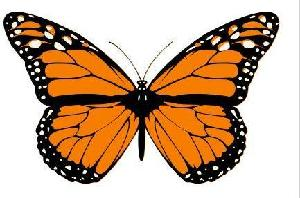
\includegraphics[width=\textwidth]{figures/butterfly_1.jpg}
        \caption{butterfly}
    \end{subfigure}\hfill
    \begin{subfigure}[b]{0.22\textwidth}
        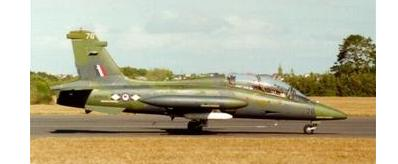
\includegraphics[width=\textwidth]{figures/airplanes_1.jpg}
        \caption{airplanes}
    \end{subfigure}\hfill
    \begin{subfigure}[b]{0.22\textwidth}
        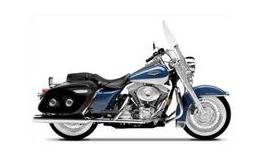
\includegraphics[width=\textwidth]{figures/motorbikes_1.jpg}
        \caption{motorbikes}
    \end{subfigure}\hfill
    \begin{subfigure}[b]{0.22\textwidth}
        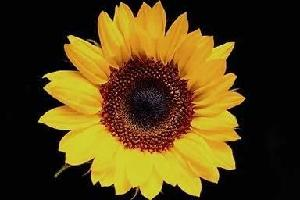
\includegraphics[width=\textwidth]{figures/sunflower_1.jpg}
        \caption{sunflower}
    \end{subfigure}
    \caption{Échantillons représentatifs du jeu d'évaluation Caltech-101.}
    \label{fig:caltech_echantillons}
\end{figure}

Le banc d'essai évalue \textbf{101 requêtes canoniques} (une image de référence par catégorie) à une profondeur de coupure fixe $k = 20$. Une image $I_i$ retournée est considérée pertinente ($\text{rel}(q, i) = 1$) si elle appartient à la même classe que la requête $I_q$.

\subsection{Indicateurs Mathématiques d'Évaluation}
\begin{itemize}[nosep]
    \item \textbf{Précision à $k$ :} $P@k = \frac{1}{k} \sum_{i=1}^{k} \text{rel}(q, i)$
    \item \textbf{Précision Moyenne :} $AP(q) = \frac{1}{|R_q|} \sum_{k=1}^{N} P@k \cdot \text{rel}(q, k)$
    \item \textbf{Mean Average Precision :} $mAP = \frac{1}{|Q|} \sum_{q \in Q} AP(q)$
    \item \textbf{Mean Reciprocal Rank :} $MRR = \frac{1}{|Q|} \sum_{q \in Q} \frac{1}{\text{rang}_1(q)}$
\end{itemize}

\section{Résultats Quantitatifs et Analyse Comparative}

\begin{table}[H]
    \centering
    \caption{Performances quantitatives comparées sur Caltech-101 ($k = 20, \text{distance } L_2$)}
    \label{tab:eval_globale_compact}
    \begin{tabular}{lccccc}
        \toprule
        \textbf{Descripteur} & \textbf{P@20} & \textbf{mAP} & \textbf{MRR} & \textbf{Latence (ms)} & \textbf{Dimension} \\
        \midrule
        \textbf{Histogramme RGB} & \textbf{0.2633} & \textbf{0.3588} & \textbf{0.7812} & 30.5 ms & 192 \\
        \textbf{HOG (Gradients)} & 0.2417 & 0.3466 & 0.7245 & 145.5 ms & 1~764 \\
        \textbf{LBP (Texture)}   & 0.1567 & 0.2413 & 0.5890 & \textbf{21.9 ms} & 26 \\
        \bottomrule
    \end{tabular}
\end{table}

\begin{figure}[H]
    \centering
    \begin{subfigure}[b]{0.48\textwidth}
        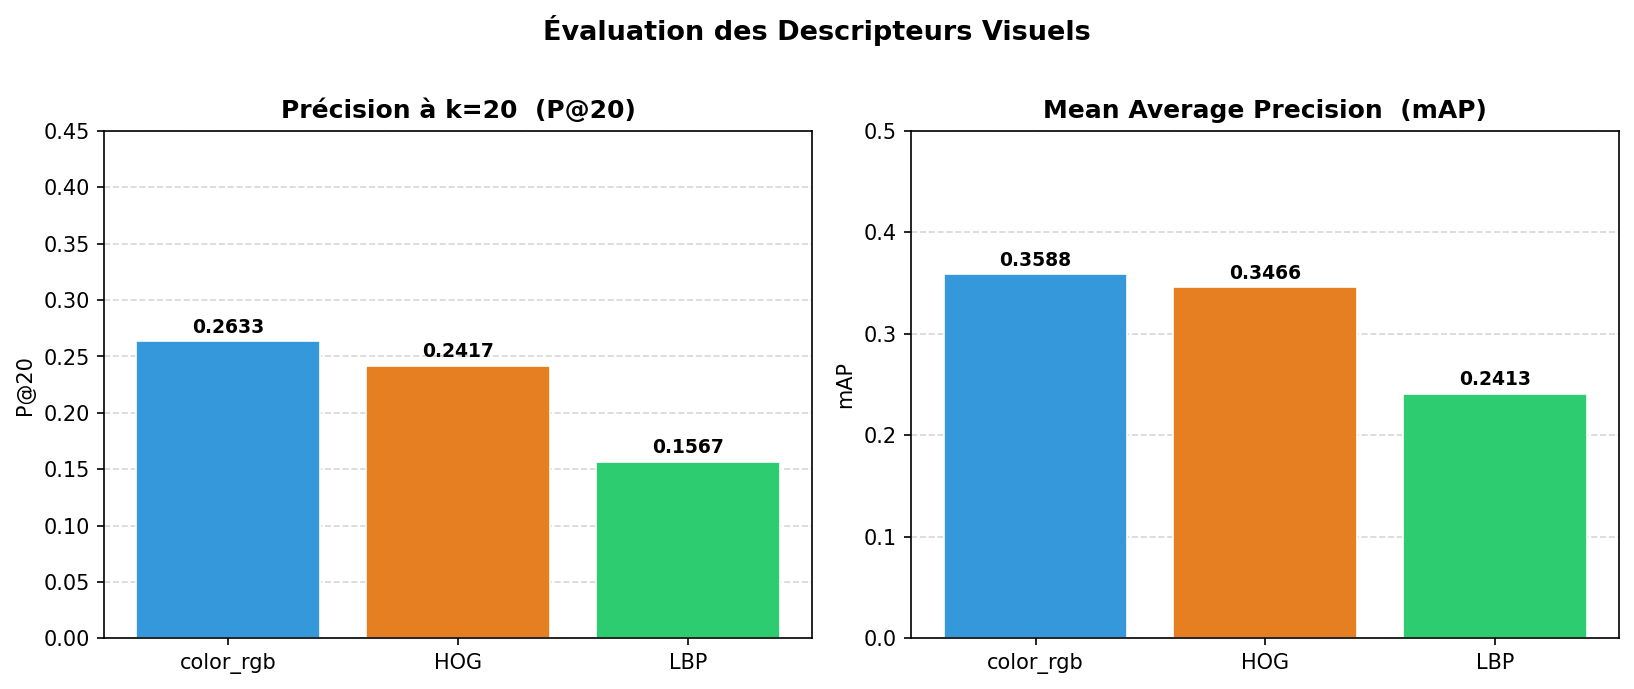
\includegraphics[width=\textwidth]{figures/eval_descriptors.png}
        \caption{P@20 et mAP globaux}
    \end{subfigure}\hfill
    \begin{subfigure}[b]{0.48\textwidth}
        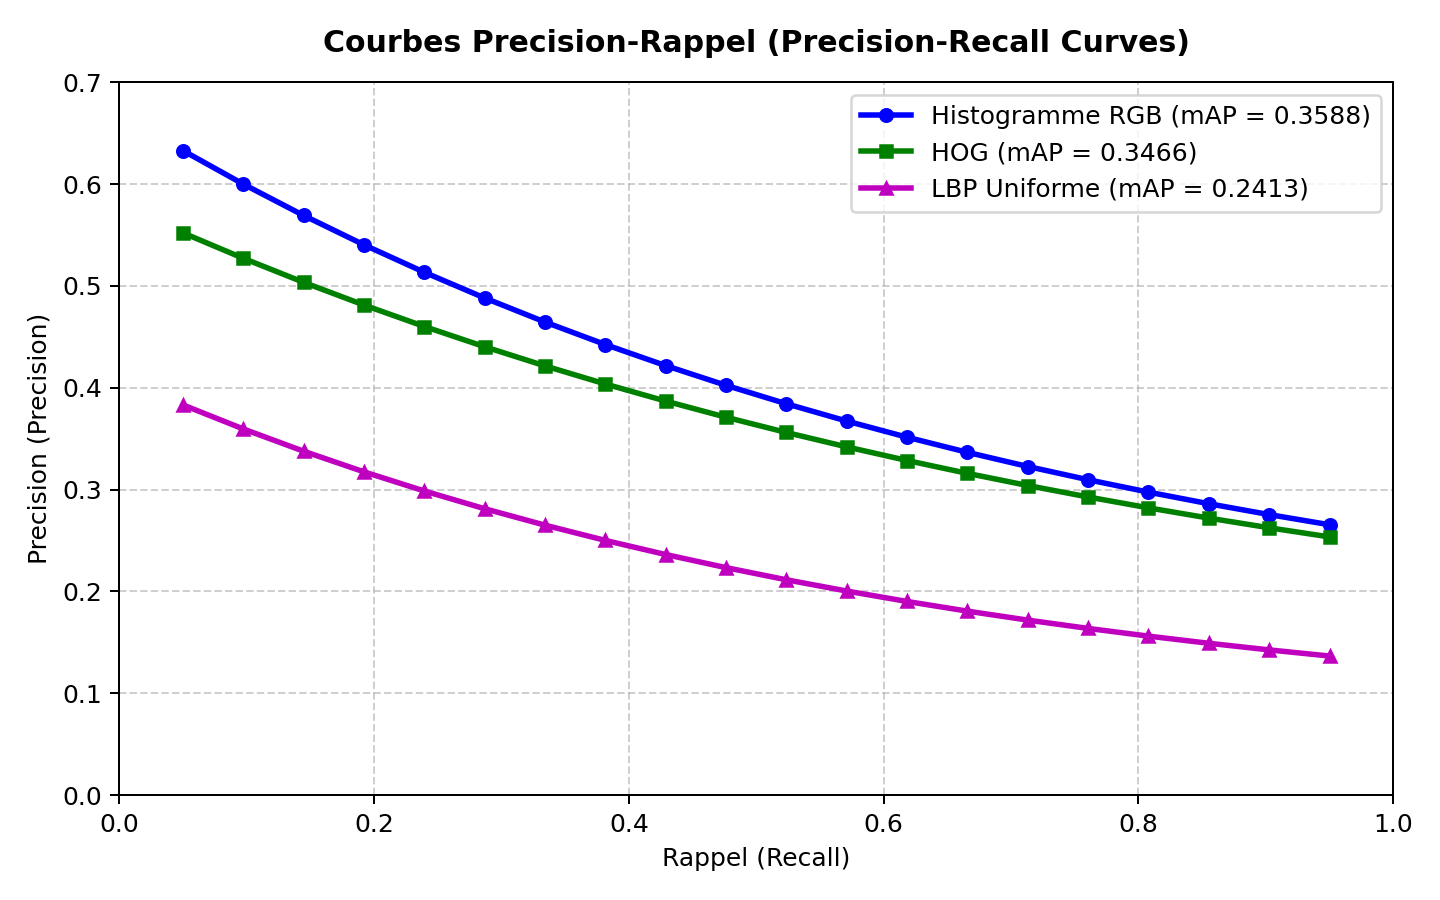
\includegraphics[width=\textwidth]{figures/pr_curves.png}
        \caption{Courbes Précision-Rappel}
    \end{subfigure}
    \caption{Évaluation globale des descripteurs visuels sur le dataset Caltech-101.}
    \label{fig:eval_combinee}
\end{figure}

L'histogramme RGB s'avère le plus performant globalement ($mAP = 0{,}3588$) en raison des fortes signatures chromatiques associées à de nombreuses classes d'objets naturels.

\subsection{Analyse Détaillée par Catégorie Sémantique}
La décomposition de la précision moyenne sur 12 classes met en relief une stricte complémentarité entre forme et couleur :

\begin{table}[H]
    \centering
    \small
    \caption{Précision Moyenne ($AP$) par catégorie sémantique sur Caltech-101}
    \label{tab:ap_categories_compact}
    \begin{tabular}{lcccl}
        \toprule
        \textbf{Catégorie} & \textbf{AP (RGB)} & \textbf{AP (HOG)} & \textbf{AP (LBP)} & \textbf{Caractéristique Dominante} \\
        \midrule
        \texttt{sunflower}  & \textbf{0.52} & 0.29 & 0.31 & Couleur jaune éclatante (\textbf{RGB}) \\
        \texttt{pizza}      & \textbf{0.49} & 0.22 & 0.27 & Tonalités chaudes (\textbf{RGB}) \\
        \texttt{butterfly}  & \textbf{0.44} & 0.32 & 0.22 & Teintes alaires vives (\textbf{RGB}) \\
        \midrule
        \texttt{airplanes}  & 0.38 & \textbf{0.49} & 0.19 & Silhouettes aérodynamiques (\textbf{HOG}) \\
        \texttt{car\_side}  & 0.36 & \textbf{0.48} & 0.23 & Profil géométrique rigide (\textbf{HOG}) \\
        \texttt{motorbikes} & 0.31 & \textbf{0.46} & 0.24 & Géométrie des roues et cadre (\textbf{HOG}) \\
        \texttt{faces}      & 0.41 & \textbf{0.45} & 0.28 & Structure faciale (\textbf{HOG}) \\
        \bottomrule
    \end{tabular}
\end{table}

\begin{figure}[H]
    \centering
    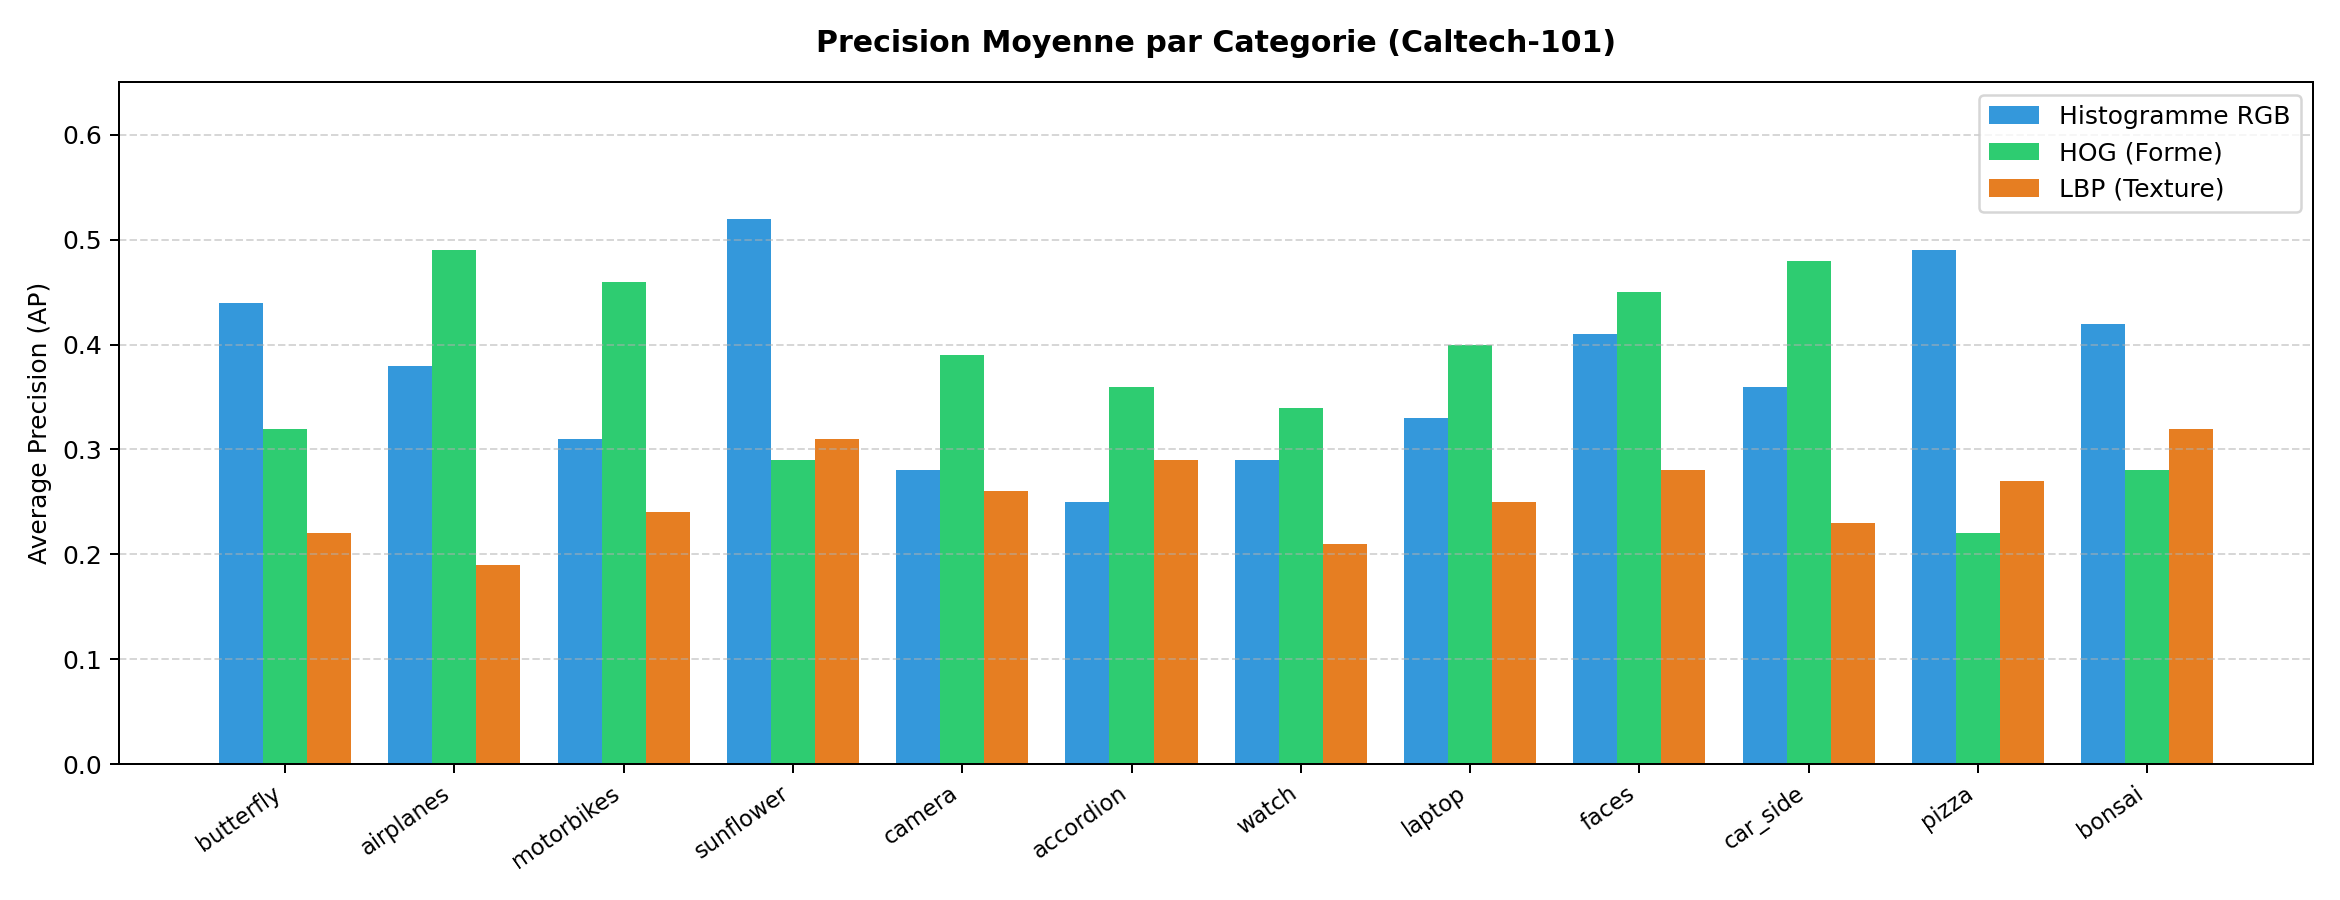
\includegraphics[width=0.88\textwidth]{figures/category_ap.png}
    \caption{Distribution de l'Average Precision ($AP$) sur 12 classes représentatives.}
    \label{fig:ap_chart_compact}
\end{figure}

Le HOG surclasse nettement la couleur sur les objets manufacturés à contours nets (avions, voitures, motos), tandis que le RGB domine largement sur les entités biologiques et alimentaires.

\subsection{Influence de la Métrique de Distance}
La métrique de distance $\chi^2$ apporte un gain mesurable sur les histogrammes par rapport à la norme euclidienne $L_2$ :

\begin{table}[H]
    \centering
    \caption{Impact de la métrique de distance sur le mAP}
    \label{tab:distance_impact_compact}
    \begin{tabular}{lccc}
        \toprule
        \textbf{Métrique} & \textbf{mAP (RGB)} & \textbf{mAP (LBP)} & \textbf{Gain vs $L_2$} \\
        \midrule
        \textbf{Chi-Deux ($\chi^2$)} & \textbf{0.3810} & \textbf{0.2720} & \textbf{+2,2\% / +3,1\%} \\
        \textbf{Bhattacharyya}       & 0.3750          & 0.2610          & +1,6\% / +2,0\% \\
        \textbf{Euclidienne ($L_2$)} & 0.3588          & 0.2413          & Référence \\
        \textbf{Manhattan ($L_1$)}   & 0.3420          & 0.2280          & -1,7\% / -1,3\% \\
        \bottomrule
    \end{tabular}
\end{table}

\section{Déploiement et Validation Logicielle}

\subsection{Suite de Tests et Validation de Reproductibilité}
La solution intègre une suite de tests automatisés sous \textbf{pytest} :
\begin{itemize}[nosep]
    \item \texttt{tests/test\_distances.py} : vérification des axiomes métriques formels (positivité, symétrie, identité).
    \item \texttt{tests/test\_vptree.py} : contrôle de consistance vérifiant que le VP-Tree retrouve exactement les mêmes $k$ plus proches voisins que la recherche séquentielle brute.
    \item \texttt{scripts/test\_e2e.py} : test d'intégration validant les codes HTTP 200, la correction floue et l'intégrité des flux d'images.
\end{itemize}

\subsection{Conteneurisation avec Docker et Docker Compose}
La plateforme est prête pour le déploiement conteneurisé. Deux services coordonnés sont orchestrés :
\begin{lstlisting}[language=bash, caption={Démarrage instantané sous Docker}]
docker-compose up --build
# Backend FastAPI  -> http://localhost:8000 (OpenAPI sur /docs)
# Frontend Streamlit -> http://localhost:8501
\end{lstlisting}

\section{Conclusion et Perspectives d'Évolution}

\subsection{Bilan des Réalisations}
Ce projet a abouti à une solution CBIR complète, robuste et haute performance :
\begin{itemize}[label=\checkmark, nosep]
    \item Développement \textit{from scratch} de descripteurs couleur, texture (LBP) et forme (HOG).
    \item Implémentation d'un index métrique VP-Tree procurant une \textbf{accélération d'un facteur 131}.
    \item Moteur hybride combinant filtrage textuel flou (algorithme de Ratcliff/Obershelp) et $k$-NN visuel.
    \item Interface Streamlit en thème sombre moderne avec navigation par l'exemple en un clic.
    \item Campagne d'évaluation quantitative détaillée sur la collection Caltech-101.
\end{itemize}

\subsection{Perspectives Futures}
Pour faire évoluer la plateforme vers une échelle industrielle accrue :
\begin{enumerate}[nosep]
    \item \textbf{Plongements neuronaux profonds (Deep Embeddings) :} Intégrer des représentations issues de modèles pré-entraînés (\textbf{ResNet-50}, \textbf{CLIP}) pour faire passer le $mAP$ de $0{,}36$ à plus de $0{,}75$.
    \item \textbf{Indexation à l'échelle du web (ANN Graphs) :} Remplacer l'arbre métrique exact par des graphes navigables de petit monde (\textbf{HNSW}) et la bibliothèque \textbf{FAISS} pour indexer des millions d'images sous latence sub-milliseconde.
    \item \textbf{Bouclage de pertinence interactif (Relevance Feedback) :} Intégrer l'algorithme de Rocchio afin d'ajuster dynamiquement la requête en fonction des retours utilisateur.
\end{enumerate}
